%1
\documentclass[aspectratio=169]{beamer}
\usetheme{Boadilla}
\usepackage[utf8]{inputenc}
\usepackage[T1]{fontenc}

\usepackage{csquotes}

\usepackage[brazilian]{babel}
\usepackage{graphicx}

\usepackage{datetime2}
\usepackage[natbib]{biblatex}

\addbibresource{bibs/bibliografia.bib}
\addbibresource{bibs/bibdoslivrosesas.bib}
\title{Software Project Canvas v1.0}
\author{Geraldo Xexéo}
\date{\today \ \DTMcurrenttime}


 \setbeamerfont{title}{series=\bfseries,size=\Huge}
\AtBeginSection[]{
  \begin{frame}
  \vfill
  \centering
  \begin{beamercolorbox}[sep=8pt,center,shadow=true,rounded=true]{title}
    \usebeamerfont{title}\insertsectionhead\par%
  \end{beamercolorbox}
  \vfill
  \end{frame}
}



\usepackage{hyperref}

\begin{document}


\begin{frame}
\titlepage
\centering
\includegraphics[width=0.4\textwidth]{imagens/alternativa3.png}
\end{frame}

%2 Sumario
\begin{frame}
\frametitle{Sumário}
\tableofcontents
\end{frame}

%3 Intro
\section{Introdução}

\begin{frame}
\frametitle{Software Project Canvas}
Uma ferramenta ágil para facilitar a colaboração das partes interessadas na definição inicial de um projeto de software.

\centering
\includegraphics[width=0.7\textwidth]{imagens/alternativa1.png}
\end{frame}


%4 Canvas
\section{O que são Canvas}

\begin{frame}
\frametitle{O que são Canvas}
Canvas são ferramentas colaborativas que ajudam no controle, decisão ou planejamento. Composta por quadros divididos em tópicos, onde informações são inseridas usando post-its.
\end{frame}

\begin{frame}
\frametitle{Exemplo: Business Model Canvas}
O \textit{Business Model Canvas} foi um dos primeiros a ser amplamente usado na indústria. Cada área recebe post-its em uma ordem definida. Exemplo:
\begin{itemize}
    \item Quadro: Customer Segments
    \item Post-it: Adolescentes praticantes de skate
\end{itemize}

\centering
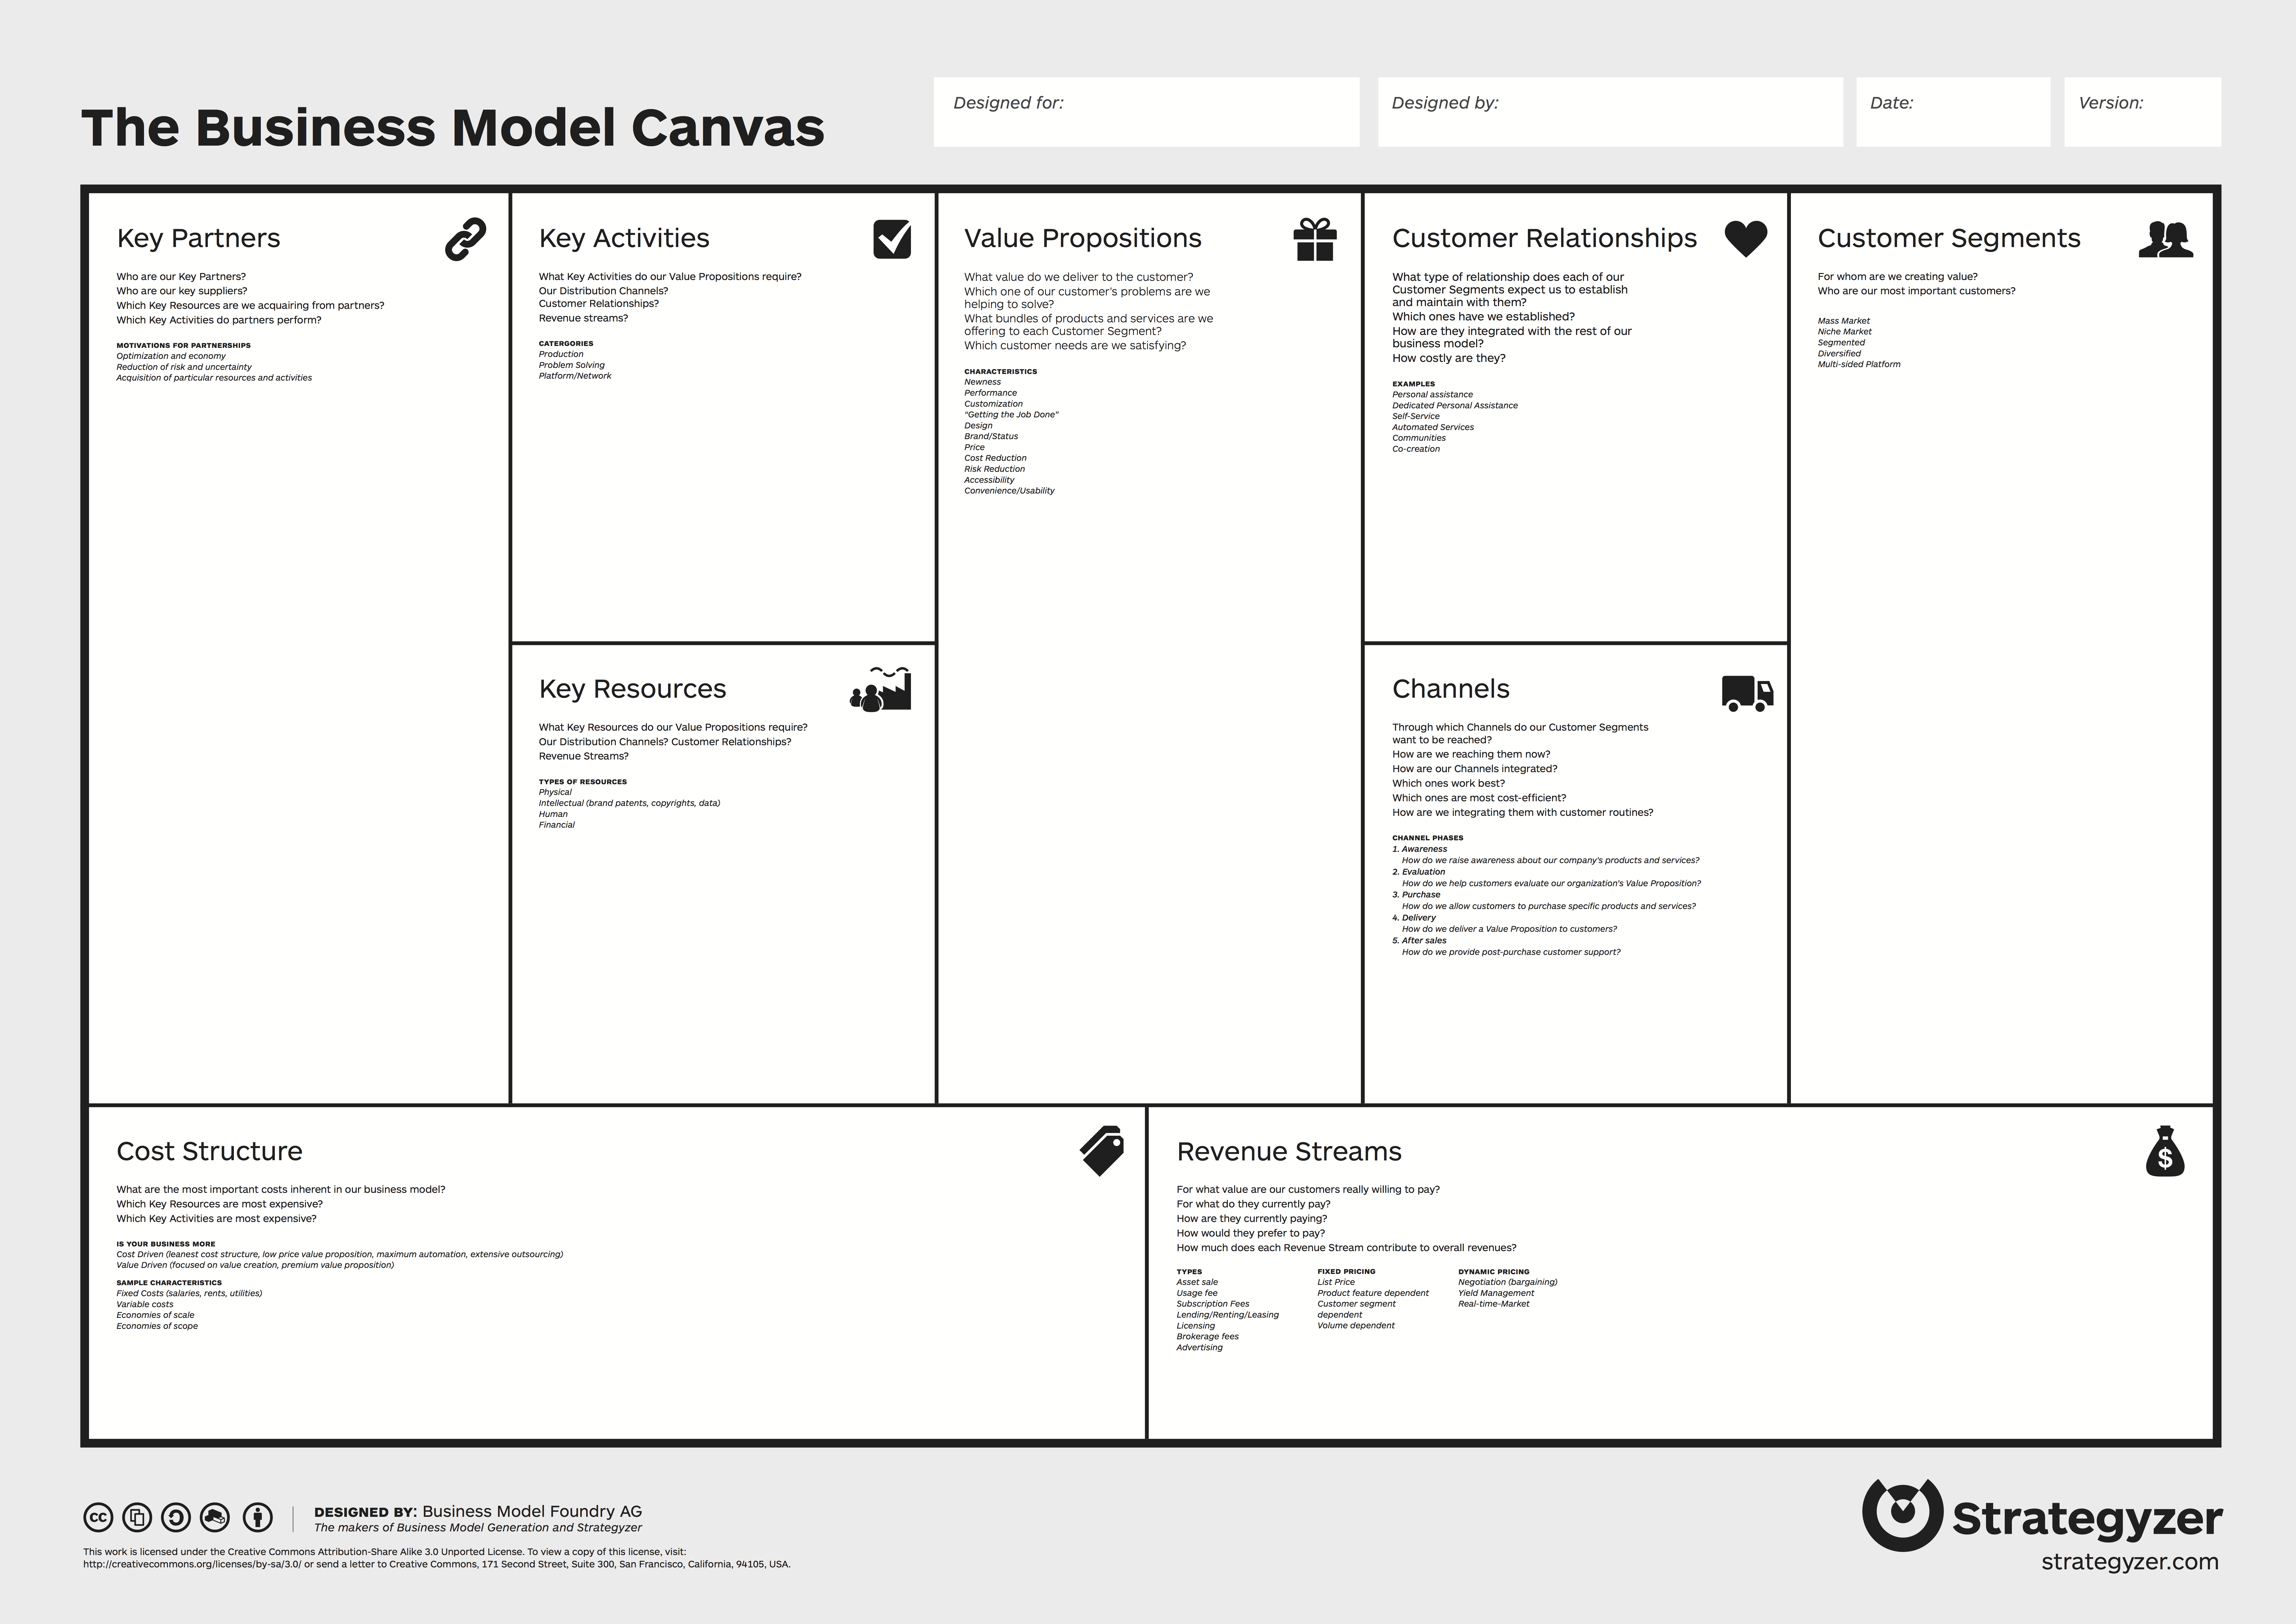
\includegraphics[width=0.5\textwidth]{imagens/BMC.png}
\end{frame}



\begin{frame}
\frametitle{O Project Model Canvas}
O \textit{Project Model Canvas}~\citep{finocchio:2013} é destinado ao planejamento inicial de projetos. Tem 12 quadros preenchidos em fases como Concepção, Integração, Revisão e Compartilhamento.

\centering
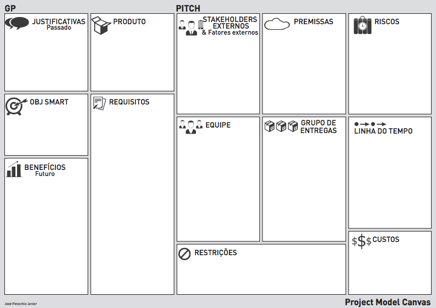
\includegraphics[width=0.5\textwidth]{imagens/ProjectMdoel Canvas.png}
\end{frame}




%5 Agilidade

\section{Projetos, Agilidade e Canvas}

\begin{frame}
\frametitle{Projetos, Agilidade e Canvas}
Gestão de Projetos visa atingir objetivos específicos de prazo, orçamento, e desempenho. Métodos ágeis oferecem maior flexibilidade e entregas incrementais, como no processo Kanban.
\end{frame}

\begin{frame}
\frametitle{O Kanban Board}
Exemplo de um quadro Kanban: divide o trabalho em tarefas a fazer, em progresso e concluídas, permitindo melhor visualização do status.
\begin{figure}
    \centering
    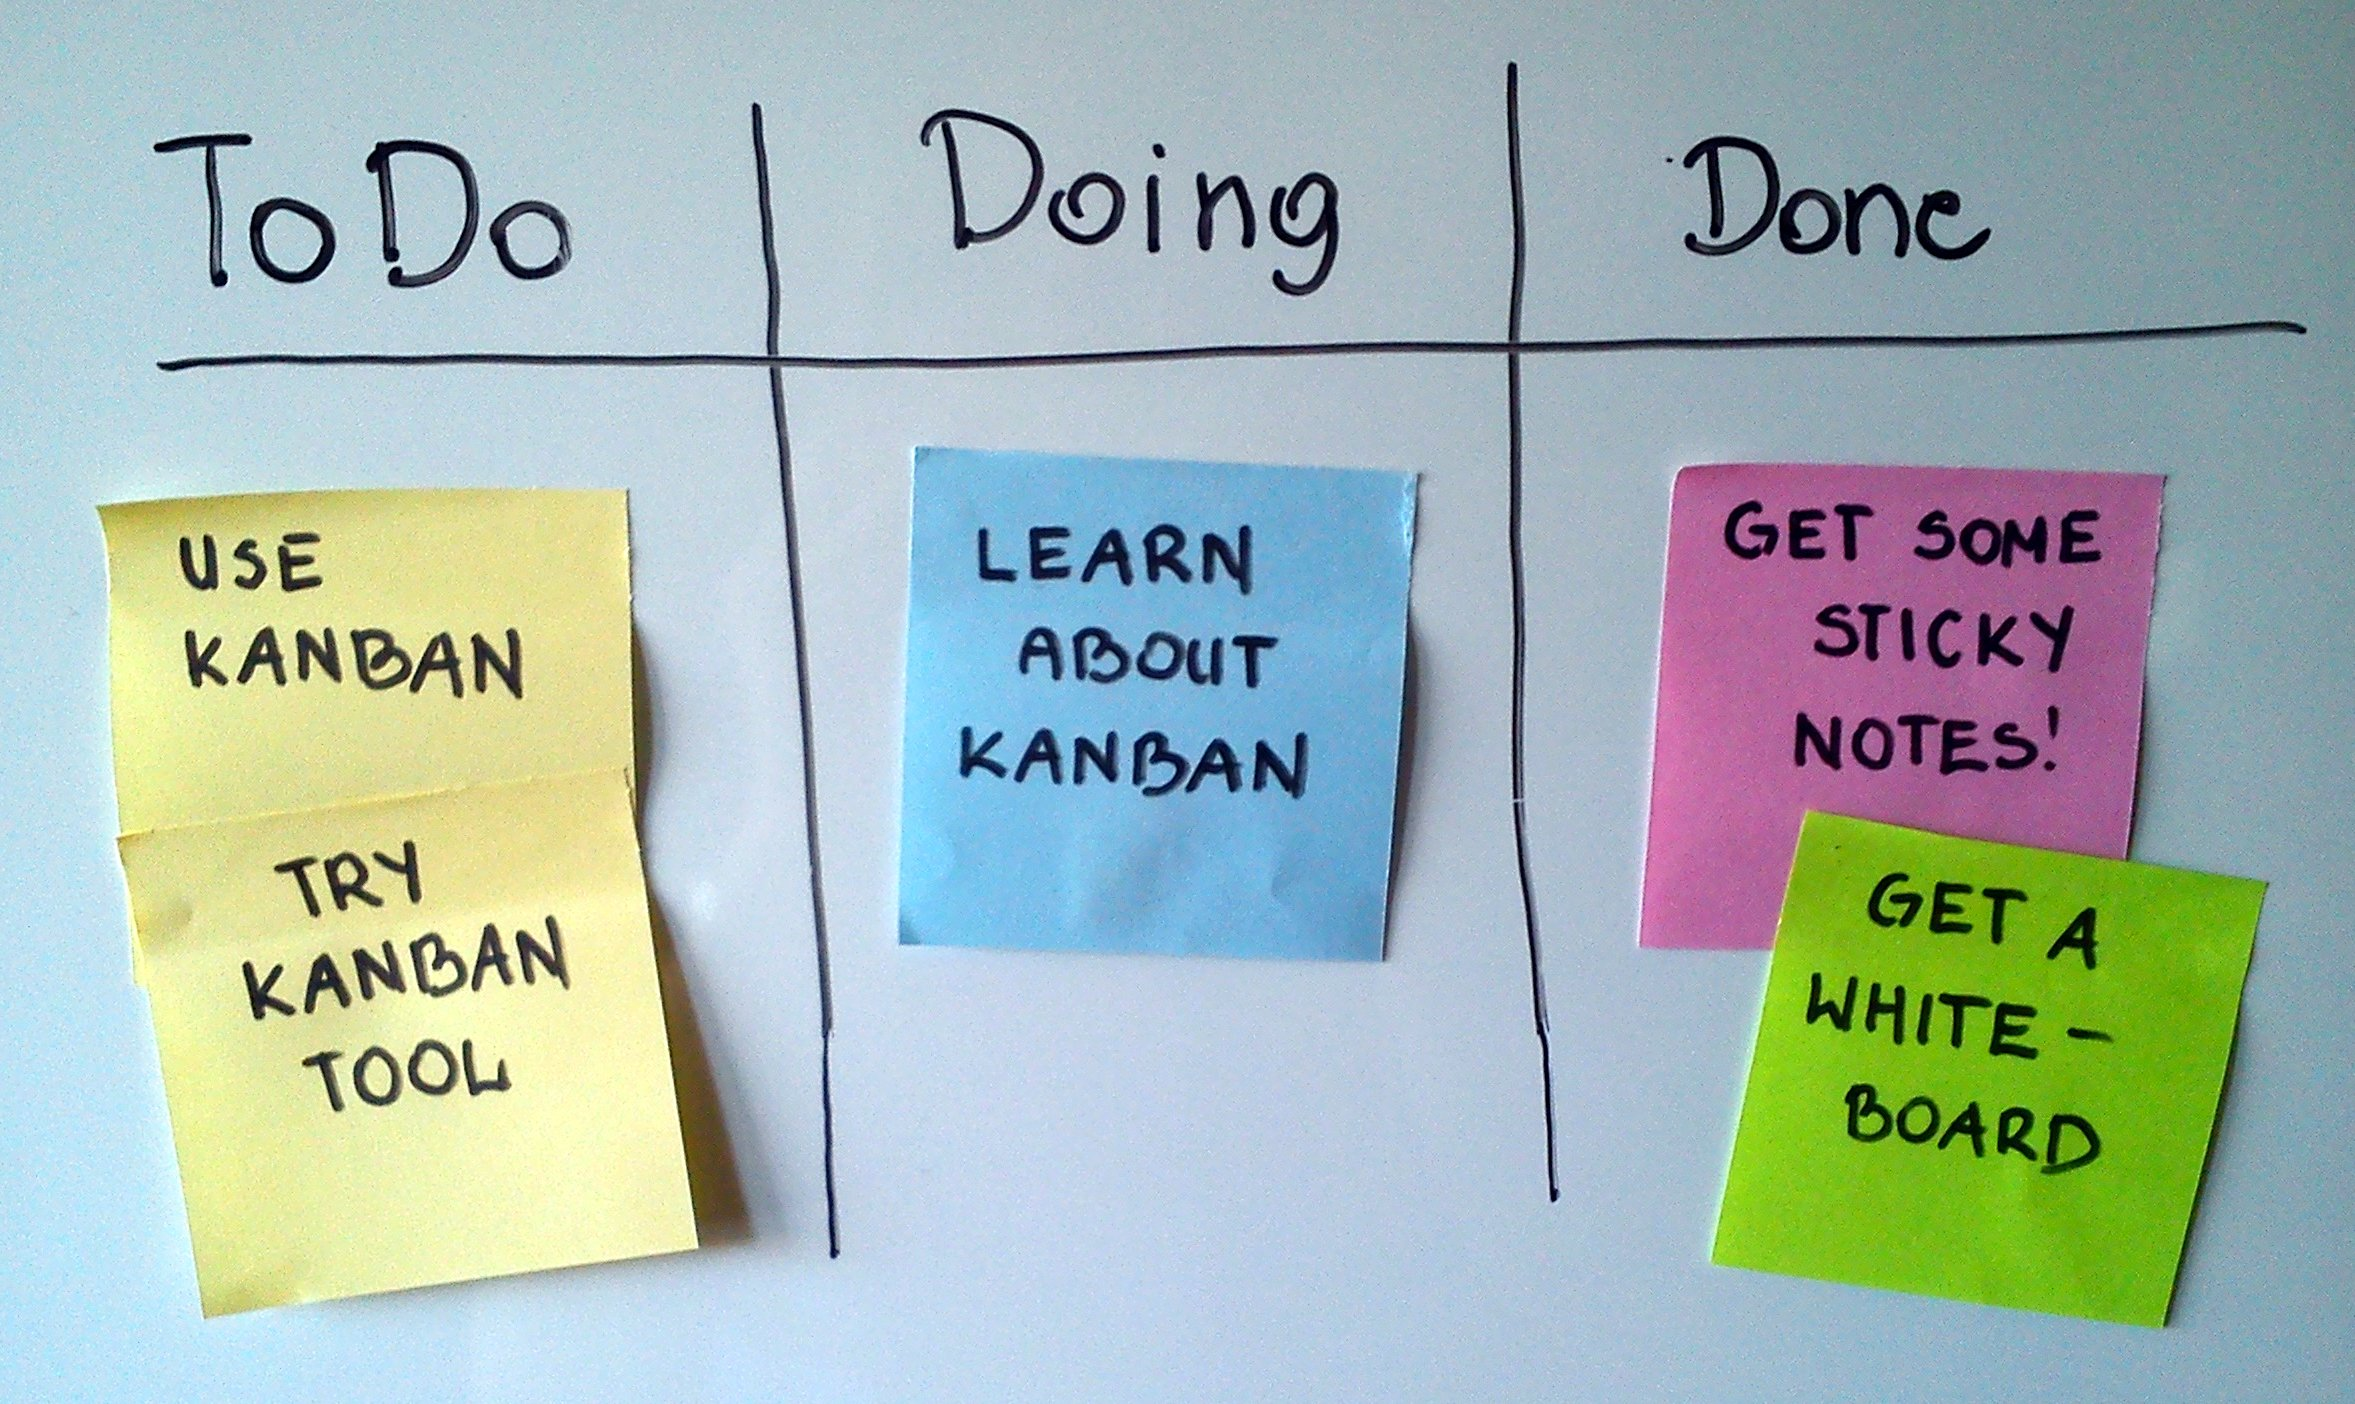
\includegraphics[width=0.7\textwidth]{imagens/Simple-kanban-board-.jpg}
    \caption{Quadro Scrum/Kanban. Fonte: Jess Iasovski, CC BY-SA 3.0}
\end{figure}
\end{frame}

% 6 SPC

\section{O Software Project Canvas}

\begin{frame}
\frametitle{O Software Project Canvas}
\begin{itemize}
    \item O Software Project Canvas utiliza 10 quadros que são organizados em 6 grupos: \textit{Why, What, Who, When, How} e \textit{How Much}.
\item Os grupos podem ser colocados em 3 ordens (alternativas 1, 2 e 3) de acrodo com o projeto.
\end{itemize}

\centering
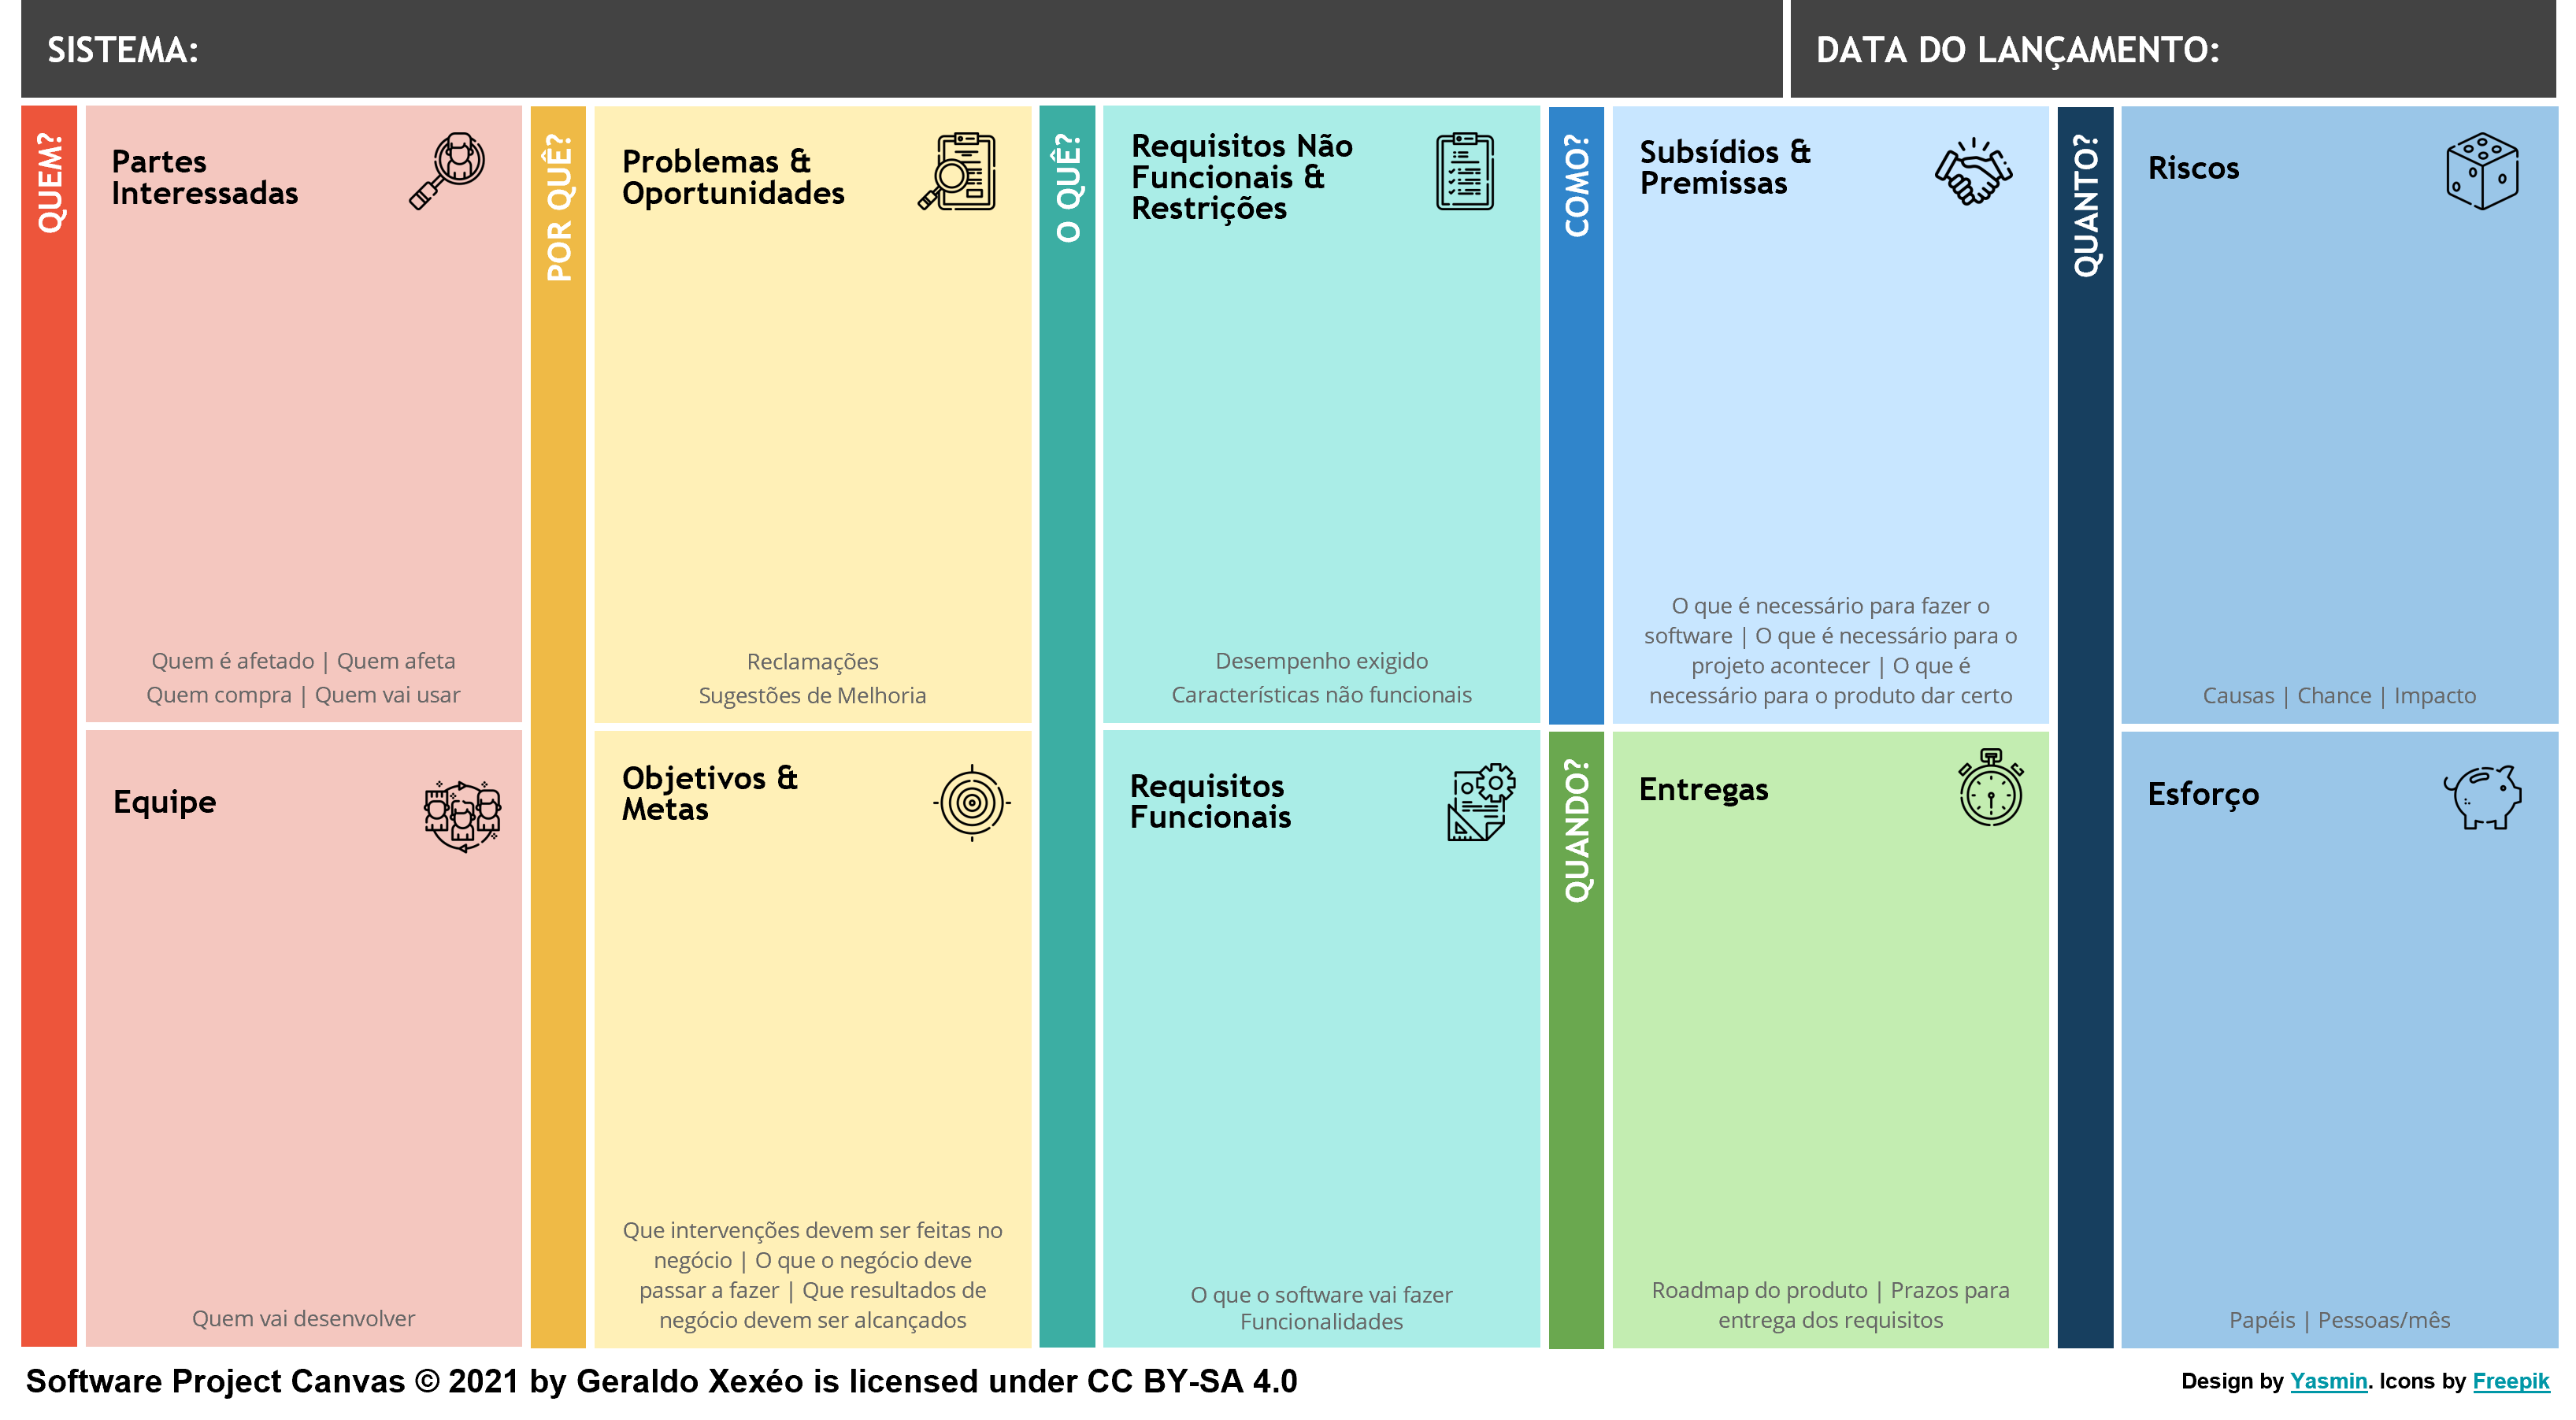
\includegraphics[width=0.5\textwidth]{dist/alternativa2.png}

\end{frame}


\begin{frame}
\frametitle{Ordem 1: Começando com o Porquê e O Quê}
\centering
\includegraphics[width=0.8\textwidth]{dist/alternativa1.png}
\end{frame}

\begin{frame}
\frametitle{Ordem 2: Começando com Quem}
\centering
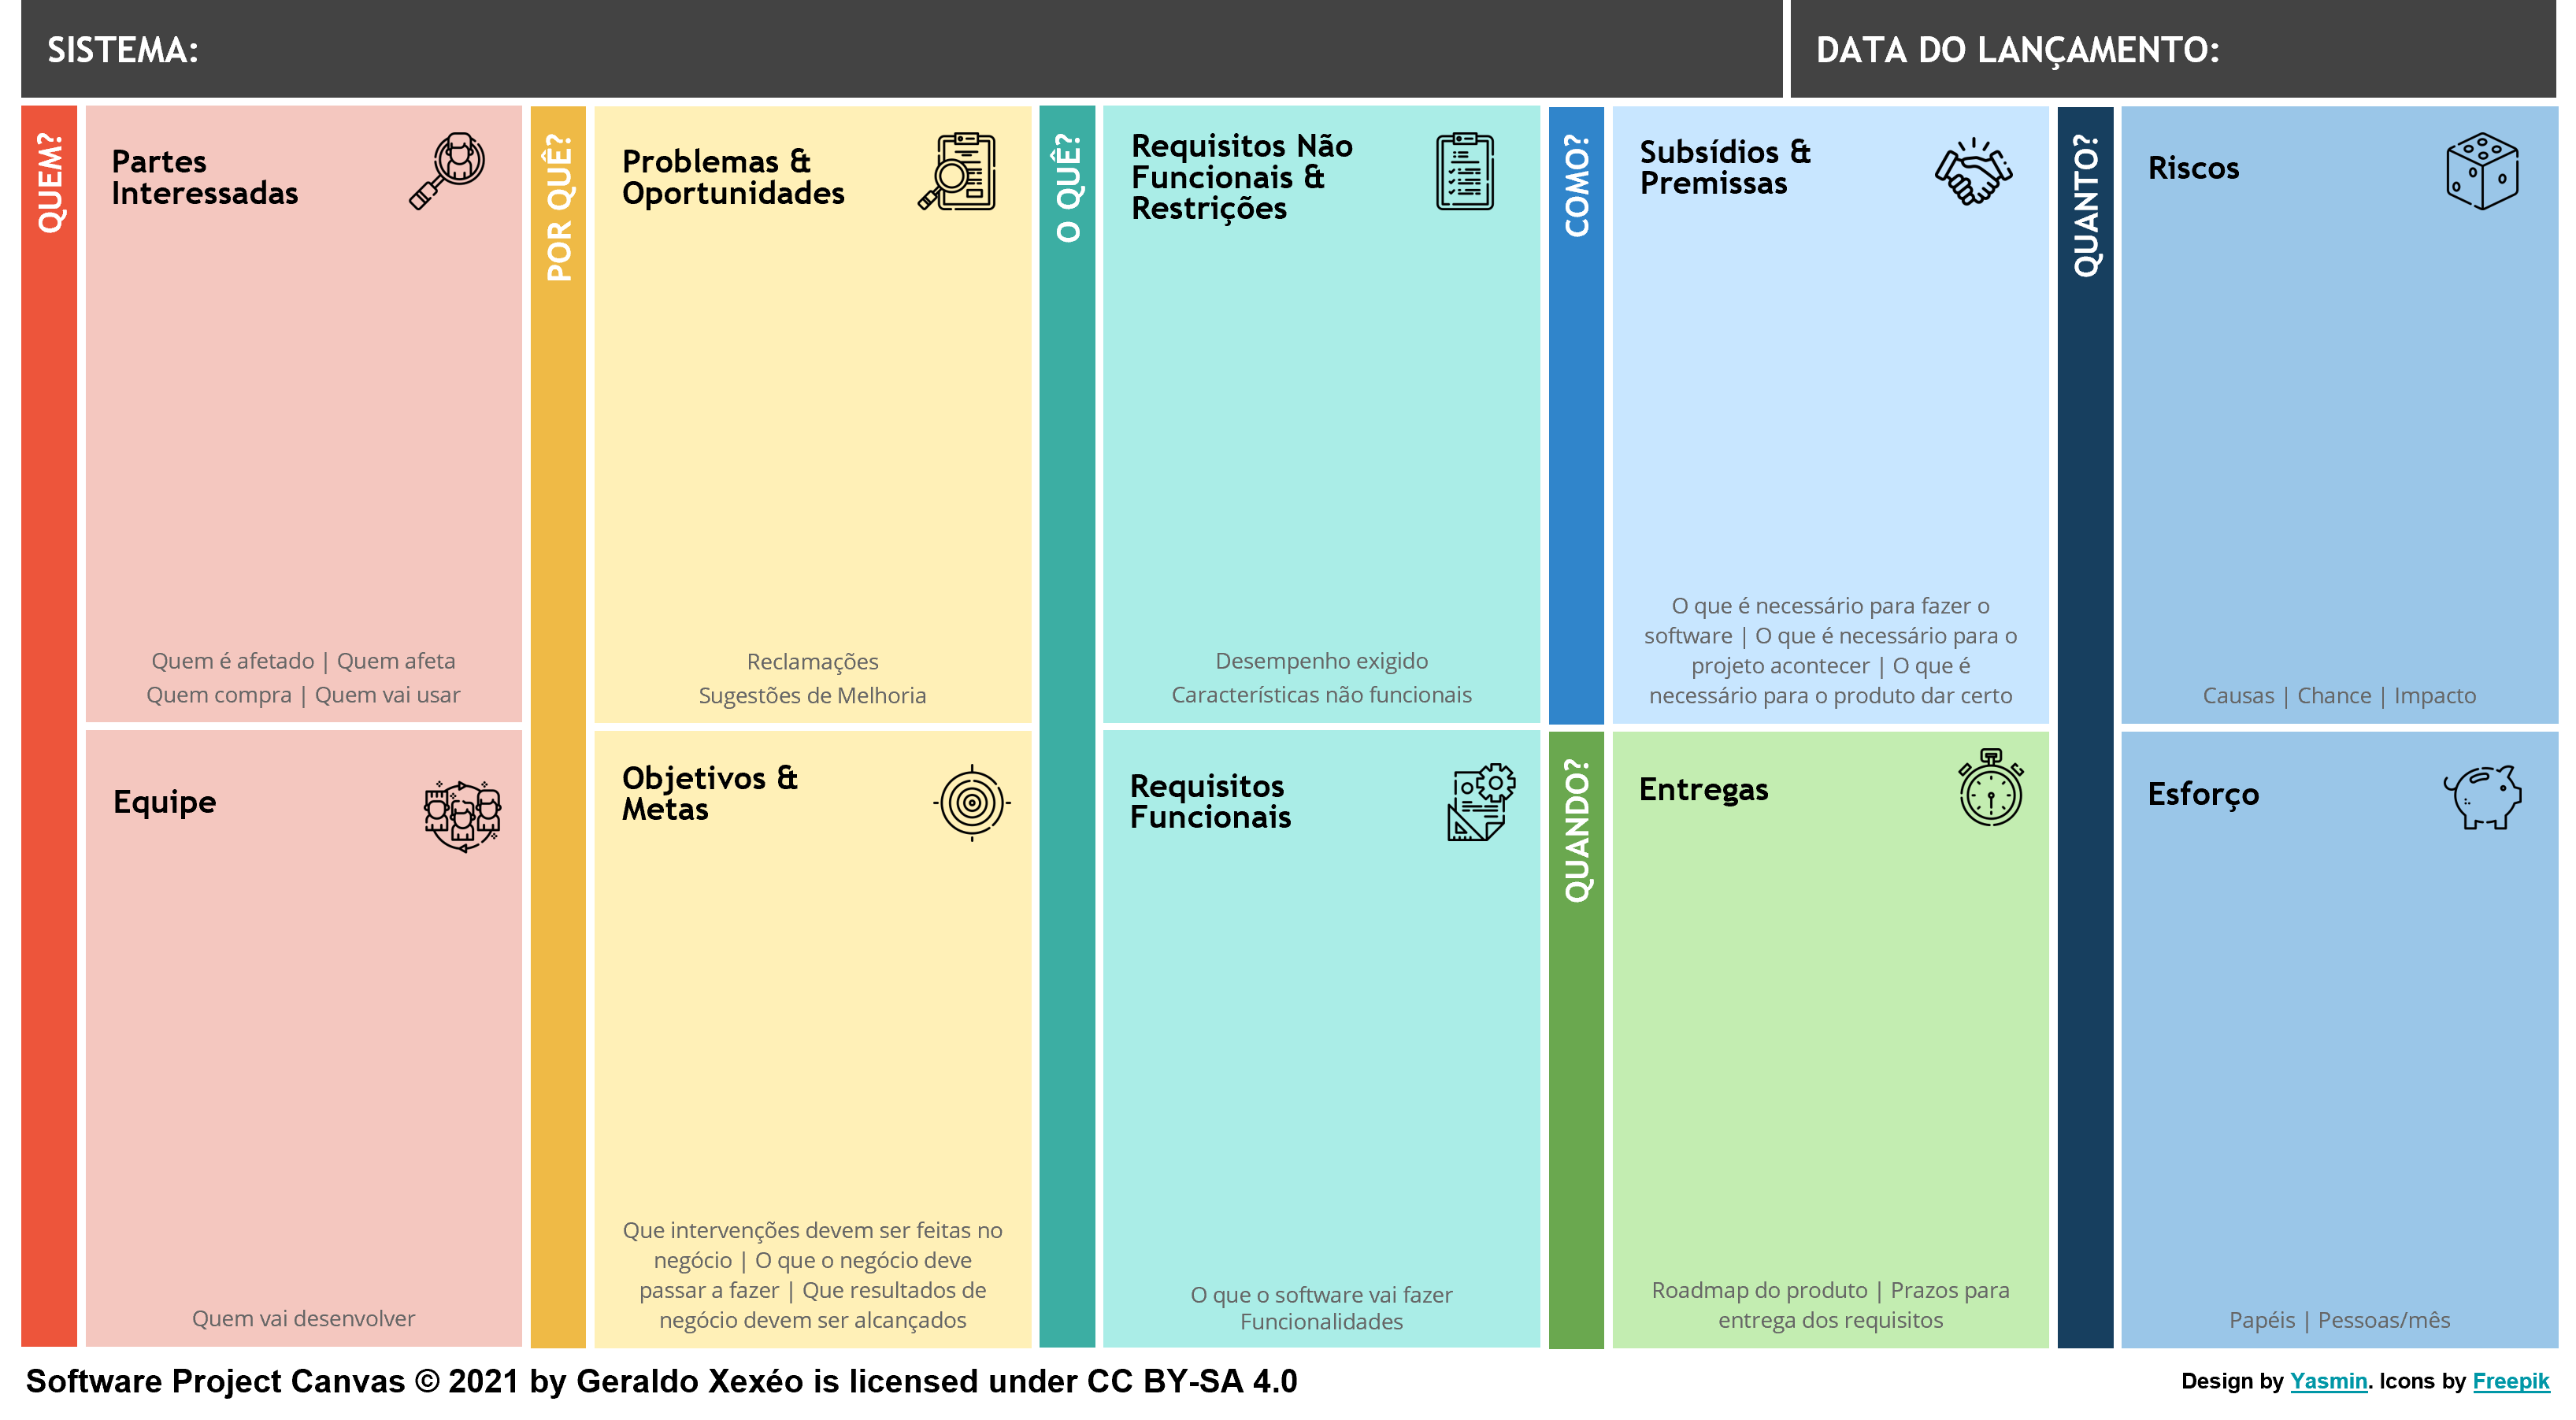
\includegraphics[width=0.8\textwidth]{dist/alternativa2.png}
\end{frame}

\begin{frame}
\frametitle{Ordem 3: Começando com Porquê e Quem}
\centering
\includegraphics[width=0.8\textwidth]{dist/alternativa3.png}
\end{frame}



\begin{frame}
\frametitle{Quadros: Por que? Problemas e Oportunidades}
\begin{columns}
        \begin{column}{.66\textwidth}
            \textbf{Problemas e Oportunidades} são identificados para justificar o projeto. Eles focam em questões como o descontentamento com o sistema atual ou a expectativa para um novo produto.
        \end{column}
        % Second column - 1/3 of the width
        \begin{column}{.33\textwidth}
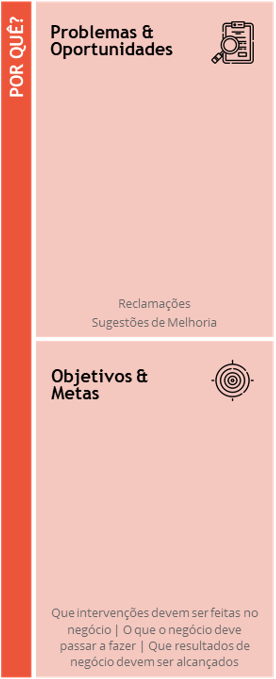
\includegraphics[height=0.7\textheight]{detalhes/Porque.png} % Replace with your image path
        \end{column}
    \end{columns}
\end{frame}

\begin{frame}
\frametitle{Quadros:  Por que? 
 Objetivos e Metas}
\begin{columns}
        \begin{column}{.66\textwidth}
        
            \textbf{Objetivos e Metas}: os objetivos são mudanças desejadas, como a construção de um sistema. As metas devem ser mensuráveis e atingíveis.


Uma das várias formas de buscar benefícios é usar a heurística IRACIS (Increase Revenue, Avoid Costs and Improve  Service)~\citep{gane:sarson:ssa,ruble_practical_1997},             

Exemplo de objetivo: detecção de necessidade de repor o estoque, com a meta diminuir reclamações sobre falta de item no estoque e as métricas: número de reclamações que um item não estava no estoque, e número de vendas perdidas porque o item não estava no estoque.


        \end{column}
        % Second column - 1/3 of the width
        \begin{column}{.33\textwidth}
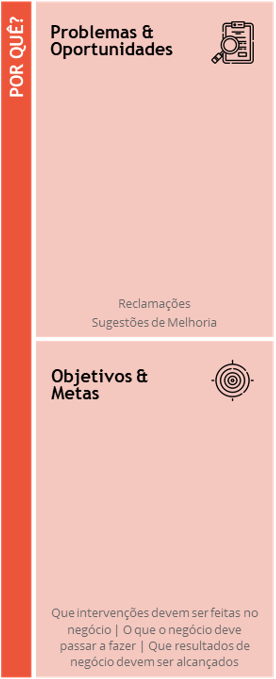
\includegraphics[height=0.7\textheight]{detalhes/Porque.png} 
        \end{column}
    \end{columns}

\end{frame}

\begin{frame}
\frametitle{Quadros: O que? Requisitos Funcionais e Não Funcionais}

\begin{columns}
    

       \begin{column}{.66\textwidth}

Um requisito é uma condição ou capacidade necessária para uma parte interessada resolver um problema ou atingir um objetivo.
       
\begin{itemize}
    \item \textbf{Requisitos Funcionais} descrevem o que o software deve fazer, enquanto os 
    \item \textbf{Requisitos Não Funcionais} falam sobre como o software deve fazer.
\end{itemize}
   
        \end{column}
        % Second column - 1/3 of the width
        \begin{column}{.33\textwidth}
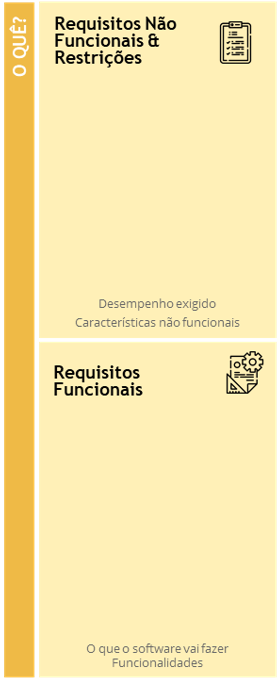
\includegraphics[height=0.7\textheight]{detalhes/Oque.png} % Replace with your image path
        \end{column}
    \end{columns}
\end{frame}


\begin{frame}
\frametitle{Taxonomia de Requisitos Não Funcionais}

    \centering
    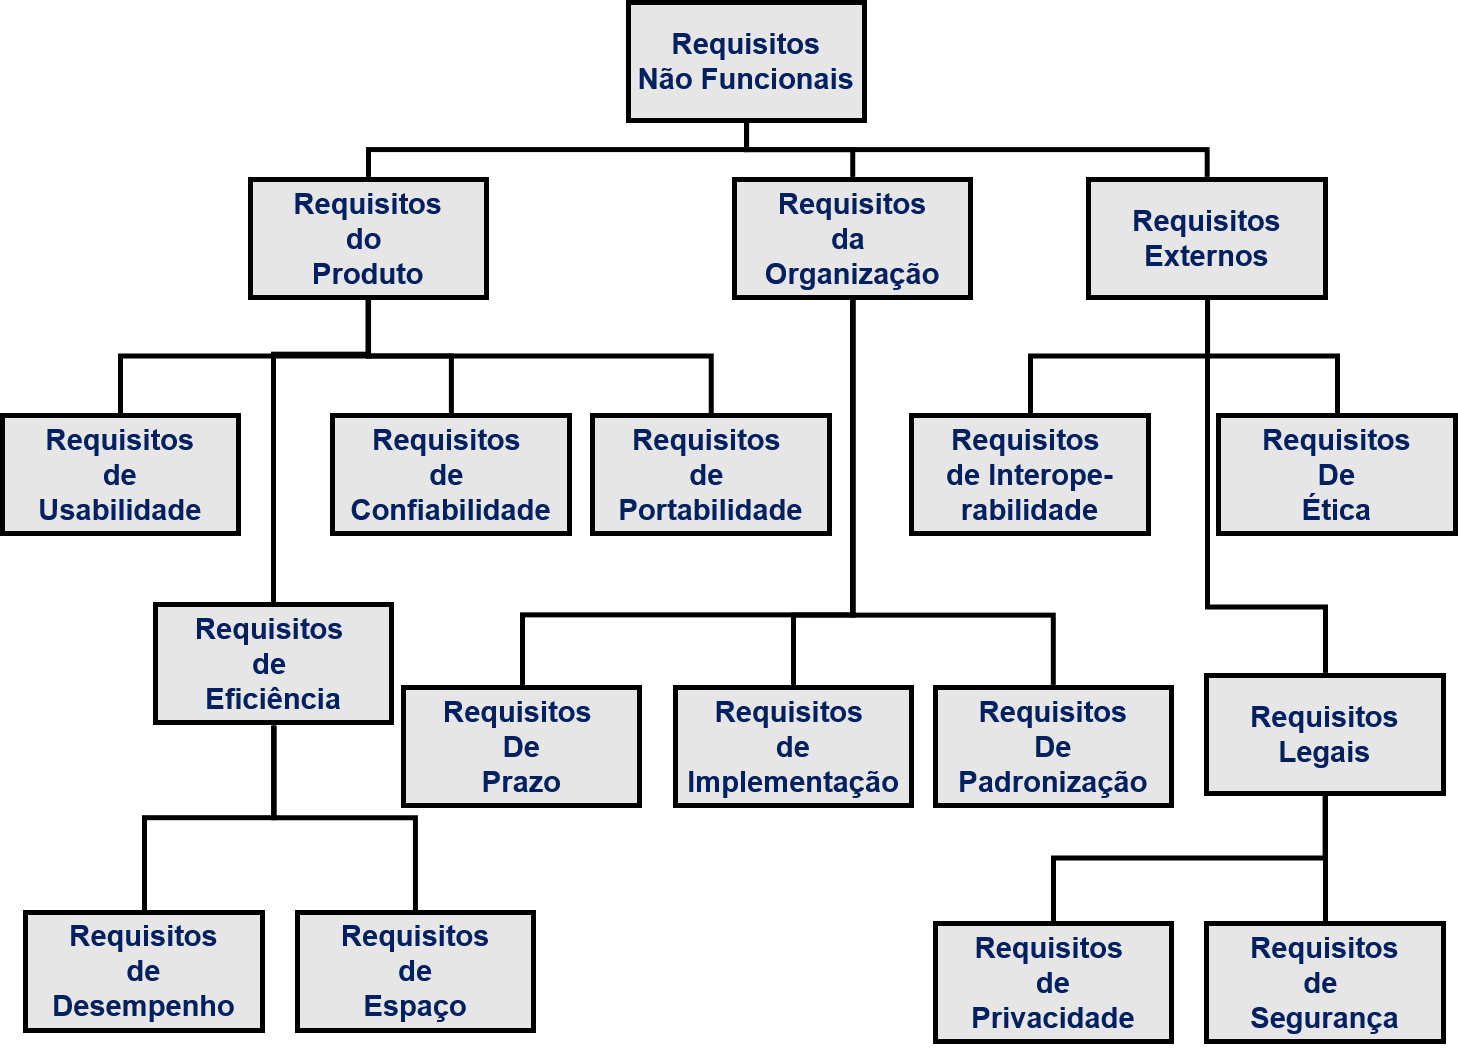
\includegraphics[width=0.6\textwidth]{imagens/NonFunReq.png}

Fonte: \citet{sommerville:software:2015}
   
\end{frame}

\begin{frame}
\frametitle{Quadros: Quem? Partes Interessadas}
\begin{columns}
    \begin{column}{.66\textwidth}
        Indivíduo, grupo ou organização que pode afetar, ser afetado, ou perceber que será afetado, por uma decisão, atividade, ou resultado, parcial ou final de um projeto
    \end{column}
    \begin{column}{.33\textwidth}
            \centering
    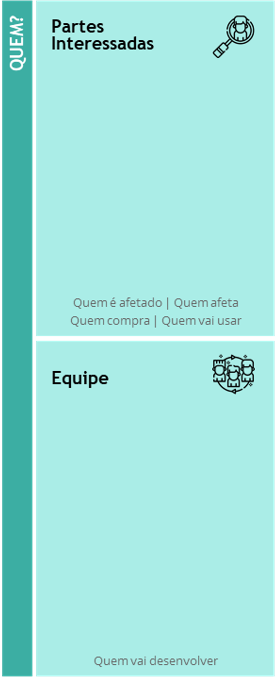
\includegraphics[width=0.6\textwidth]{detalhes/quem.png}
    \end{column}
\end{columns}

    
\end{frame}


\begin{frame}
\frametitle{Quadros: Quem? Equipe}
\begin{columns}
    \begin{column}{.66\textwidth}
Nesse quadro é indicada a equipe necessária para o desenvolvimento do projeto. Cada \textit{post-it} deve indicar um papel a ser tomado pelos membros da equipe. Quando for necessário mais de uma pessoa, isso deve ser indicado no mesmo \textit{post-it}. Possivelmente, algumas pessoas podem estar nomeadas no mesmo \textit{post-it}, ou em outro, de outra cor, possivelmente menor, colocado sobre o primeiro.
    \end{column}
    \begin{column}{.33\textwidth}
            \centering
    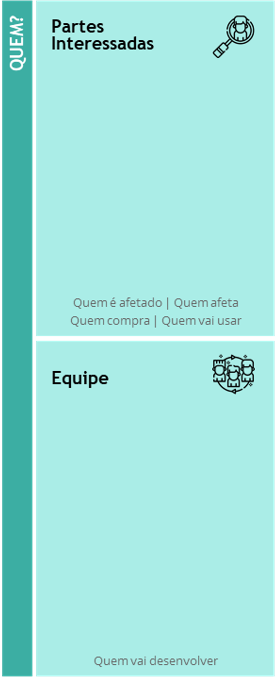
\includegraphics[width=0.6\textwidth]{detalhes/quem.png}
    \end{column}
\end{columns}
\end{frame}


\begin{frame}
\frametitle{Quadros: Como? Subsídios e Premissas}
\begin{columns}
    \begin{column}{.66\textwidth}
Tudo que é necessário para que o projeto tenha sucesso.

Premissas e subsídios são garantidas pelas partes interessadas, em favor da equipe. Caso uma parte interessada não cumpra seu compromisso em garantir a premissa, ocorre um risco do projeto.

    \end{column}
    \begin{column}{.33\textwidth}
            \centering
    \includegraphics[width=0.6\textwidth]{detalhes/como.png}
    \end{column}
\end{columns}

    
\end{frame}

\begin{frame}
\frametitle{Quadros: Quando? Entregas}
\begin{columns}
    \begin{column}{.66\textwidth}
Um projeto de software moderno é feito de forma iterativa e incremental~\citep{pressman:2019,essential:scrum}, o que implica em várias pequenas entregas, que se iniciam com protótipos, provas de conceito ou um produto mínimo viável, e se seguem de versões ou \textit{releases} que fornecem cada vez mais valor aos seus usuários.
    \end{column}
    \begin{column}{.33\textwidth}
            \centering
    \includegraphics[width=0.6\textwidth]{detalhes/quando.png}
    \end{column}
\end{columns} 
\end{frame}


\begin{frame}
\frametitle{Quadros: Quanto? Riscos}
\begin{columns}
    \begin{column}{.66\textwidth}
Riscos são incertezas que podem influenciar o resultado do projeto. Atualmente riscos são divididos em ameaças e oportunidades, isto é, existem riscos negativos e positivos.
    \end{column}
    \begin{column}{.33\textwidth}
            \centering
    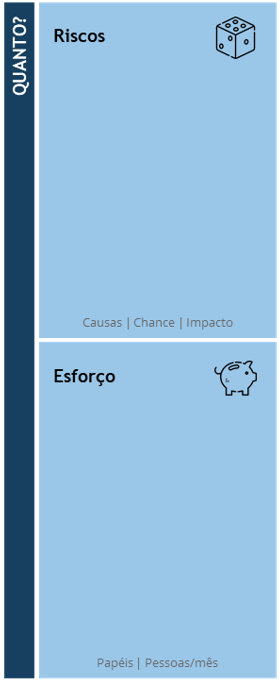
\includegraphics[width=0.6\textwidth]{detalhes/quanto.png}
    \end{column}
\end{columns} 
\end{frame}

\begin{frame}
\frametitle{Quadros: Quanto? Esforço}
\begin{columns}
    \begin{column}{.66\textwidth}
Esforço para desenvolver o software em homens-mês ou homem hora. No momento da reunião onde o canvas é usado, não é possível ainda usar uma técnica fortemente quantitativa para isso, pois não se espera que seja possível nem estimar o tamanho real do software, então isso deve ser feito a partir da experiência do grupo, com comparações com projetos anteriores.
    \end{column}
    \begin{column}{.33\textwidth}
            \centering
    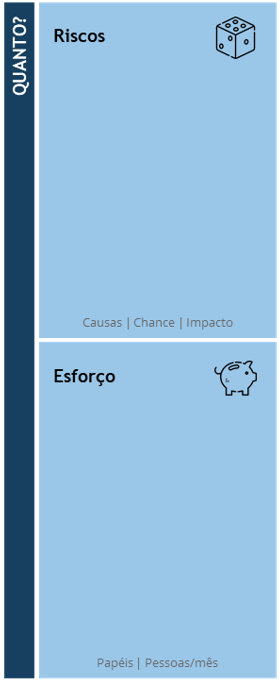
\includegraphics[width=0.6\textwidth]{detalhes/quanto.png}
    \end{column}
\end{columns} 
\end{frame}


% 7 Metodologia 
\section{Metodologia do Software Project Canvas}

\begin{frame}

\frametitle{A Metodologia do SPC}

\centering
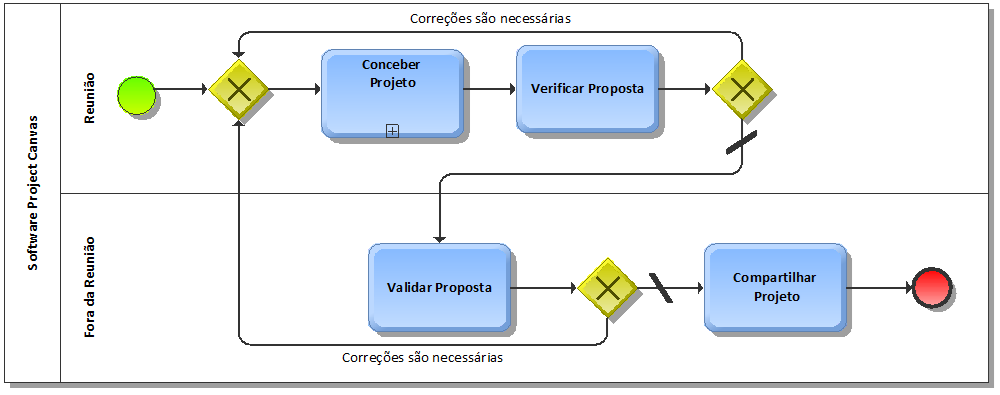
\includegraphics[width=\textwidth]{imagens/Software Project Canvas - 4 pessos.adf.png}
    
\end{frame}

\begin{frame}
\frametitle{Metodologia: Conceber Projeto}
O projeto é concebido em reuniões facilitadas, onde representantes discutem e preenchem os quadros do Canvas. A estratégia usada é a de divergência e convergência de ideias.
\end{frame}

\begin{frame}
\frametitle{Conceber Projeto: Passo a Passo}
    \centering
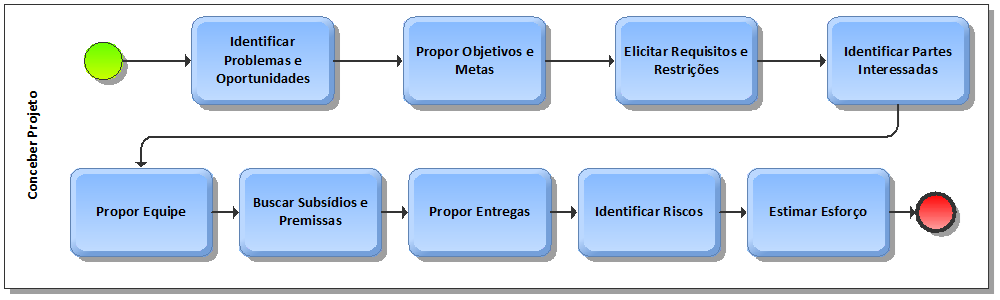
\includegraphics[width=\textwidth]{imagens/Conceber Projeto do Software Project Canvas.png}
\end{frame}

\begin{frame}
\frametitle{Metodologia: Verificar Proposta}
A verificação envolve uma análise detalhada para garantir que o Canvas está coeso e atende às necessidades das partes interessadas.
\end{frame}

\begin{frame}
\frametitle{Metodologia: Validação e Compartilhamento}
Após verificação, o Canvas é validado com outras partes da organização. O compartilhamento pode ser feito por meio de workshops, documentos ou reuniões.
\end{frame}




%8 Conclusão

\section{Conclusão}

\begin{frame}
\frametitle{Conclusão}
O Software Project Canvas facilita o planejamento inicial de projetos de software. Ele foi ajustado para atender melhor às necessidades específicas da Engenharia de Software.
\end{frame}


% 9 extras 

\section*{Agradecimentos}

\begin{frame}
\frametitle{Agradecimentos}
Agradeço a Yasmin pelo design final do \textit{Software Model Canvas}, e aos alunos Eduardo Mangeli e Marcus Parreira pelas críticas e sugestões.
\end{frame}



\section*{Licença}
\begin{frame}
\begin{figure}[h]
    \centering
    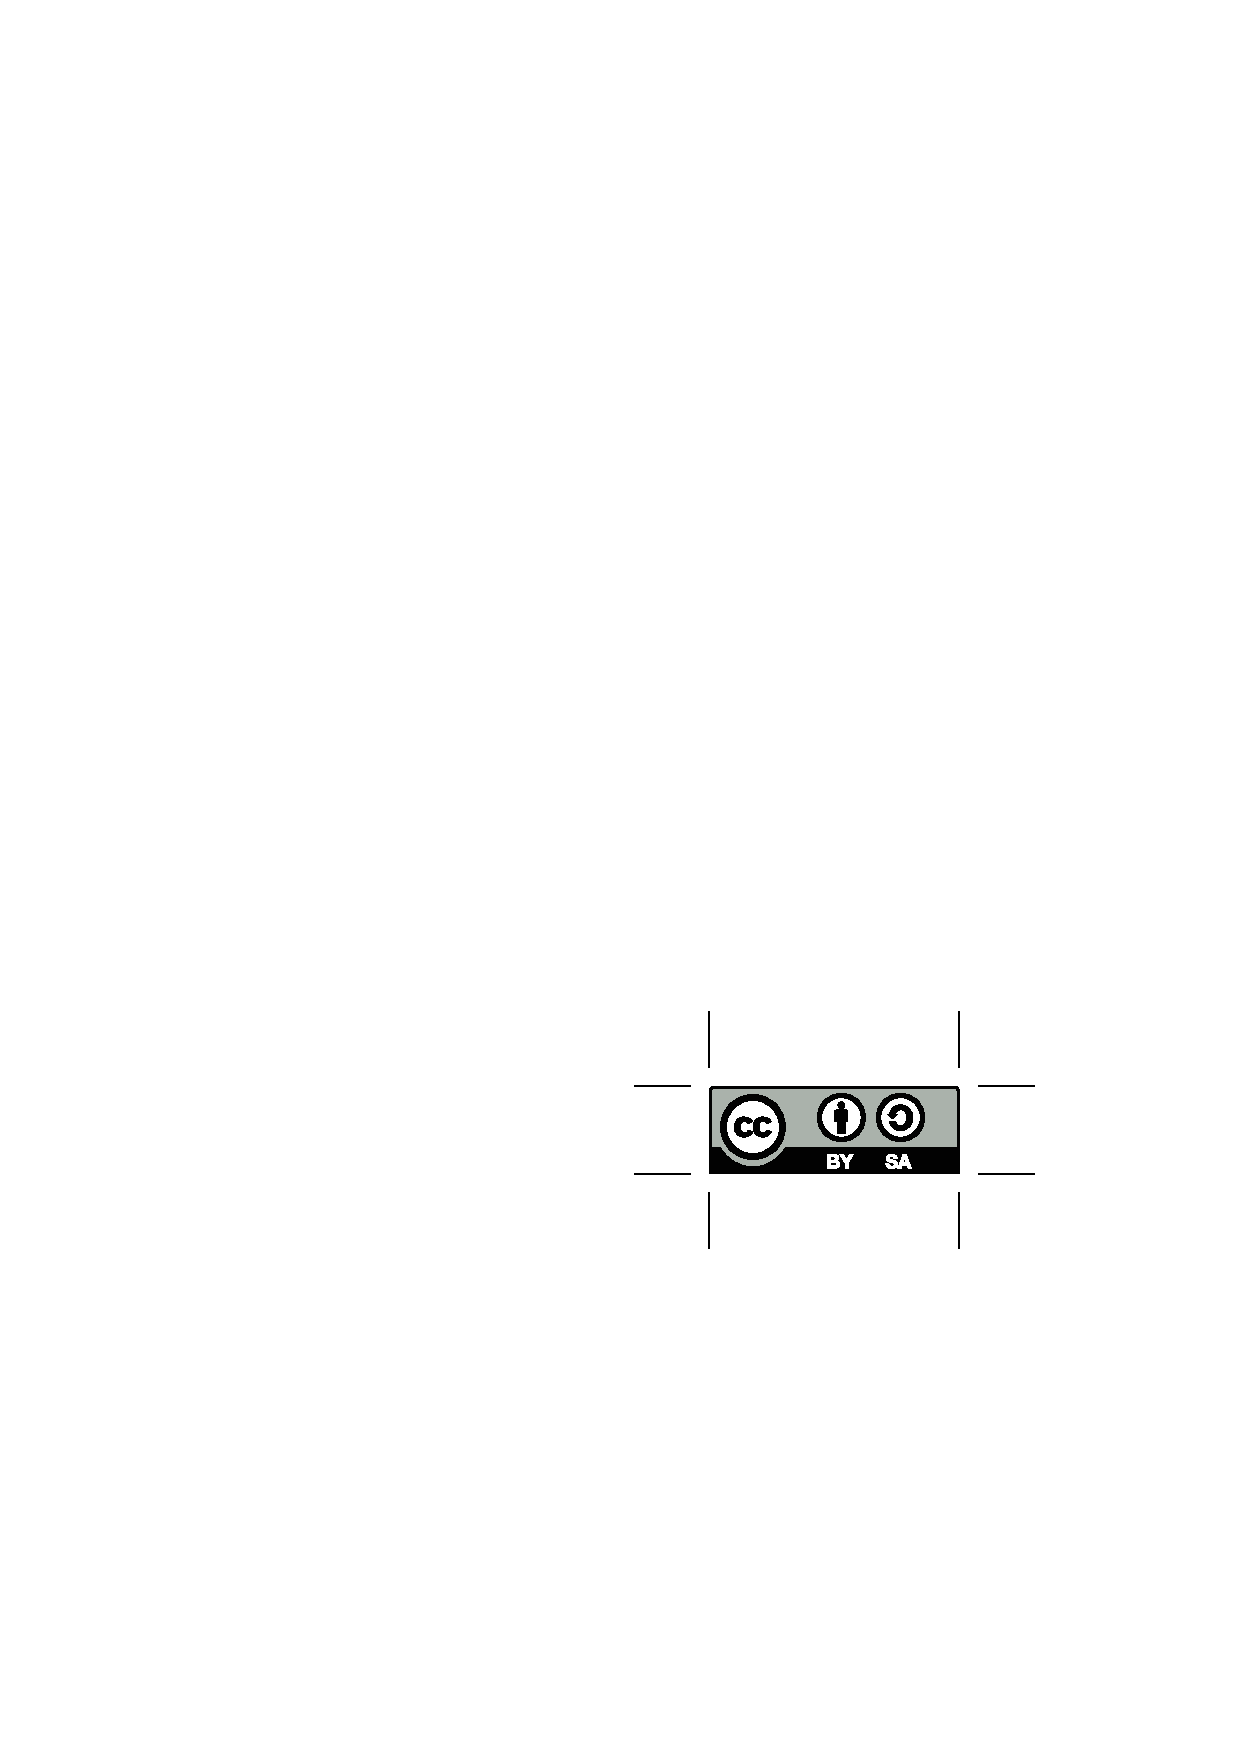
\includegraphics{imagens/by-sa}
    \label{fig:by-sa}
\end{figure}


Software Model Canvas Copyright \copyright\  2021,2024 Geraldo Xexéo está licenciado com uma Licença Creative Commons - Atribuição-CompartilhaIgual 4.0 Internacional.

Baseado no trabalho disponível em:

\url{https://github.com/xexeo/Software-Project-Canvas}.

Podem estar disponíveis autorizações adicionais às concedidas no âmbito desta licença com \url{email:xexeo@ufrj.br}.

O texto completo da licença pode ser obtido em:
\url{https://creativecommons.org/licenses/by-sa/4.0/}

\end{frame}

\end{document}




